\section{Introduction}
This section covers how the research was put into practice, with a particular emphasis on how machine learning models were put into practice and how they were integrated into a working web application for \gls{fer}.
\section{Artificial Intelligence and Machine Learning}
The preparation of datasets, the training environment, and the computational resources employed will be discussed in the following section.
Providing specific details about the measures taken to guarantee that the data was suitable for learning, the augmentation methods used to improve model performance, and the training approaches used to maximize model performance.
The evaluation metrics and the outcome of testing the models on hypothetical data are also included in this \gls{ml} section.
\subsection{Setup and Preparation}
\subsubsection{Environment Setup}
The models are developed with a robust software environment designed for advanced \gls{ml} tasks.
The preferred programming language was Python \citep{python_2019_python}, which is well-known for its adaptability and power in data manipulation and machine learning.
Then, the research and model training were carried out with Jupyter Notebook \citep{jupyter_2019_project}, which is an interactive computing environment that enables real-time code execution, analysis and visualization.
The libraries used for model training are listed below.
\begin{itemize}
    \item \textbf{Keras}: Chosen for its user-friendly API which operates on top of TensorFlow, it enabled to build and train neural network models with relative ease. \citep{team_keras}
    \item \textbf{NumPy}: It is used for handling of numerical operations on array, forming the foundation of data structures in \gls{ml} tasks. \citep{numpy_2009_numpy}
    \item \textbf{Pandas}: This library provided robust data manipulation and cleaning capabilities which makes organizing tabular data and dataset transformation more easier. \citep{pandas_2018_python}
    \item \textbf{Scikit-learn (sklearn)}: A broad range of machine learning tools, including cross-validation methods, model assessment, and preprocessing, are available in this library and aid in the improvement of learned models. \citep{scikitlearn_2019_scikitlearn}
    \item \textbf{OpenCV (cv2)}: This library provided extensive image processing capabilities, which were crucial in manipulating and preparing facial images for training. \citep{opencv_2019_opencv}
    \item \textbf{Matplotlib and Seaborn}: These libraries were used for data visualization. They allow findings to be converted into charts, which provide further insight into the functioning of the models. \citep{matplotlib_2012_matplotlib} \citep{seaborn_2012_seaborn}
\end{itemize}
\subsubsection{Data Preparation}
\paragraph{Data Collection}
\begin{figure}[h!]
    \centering
    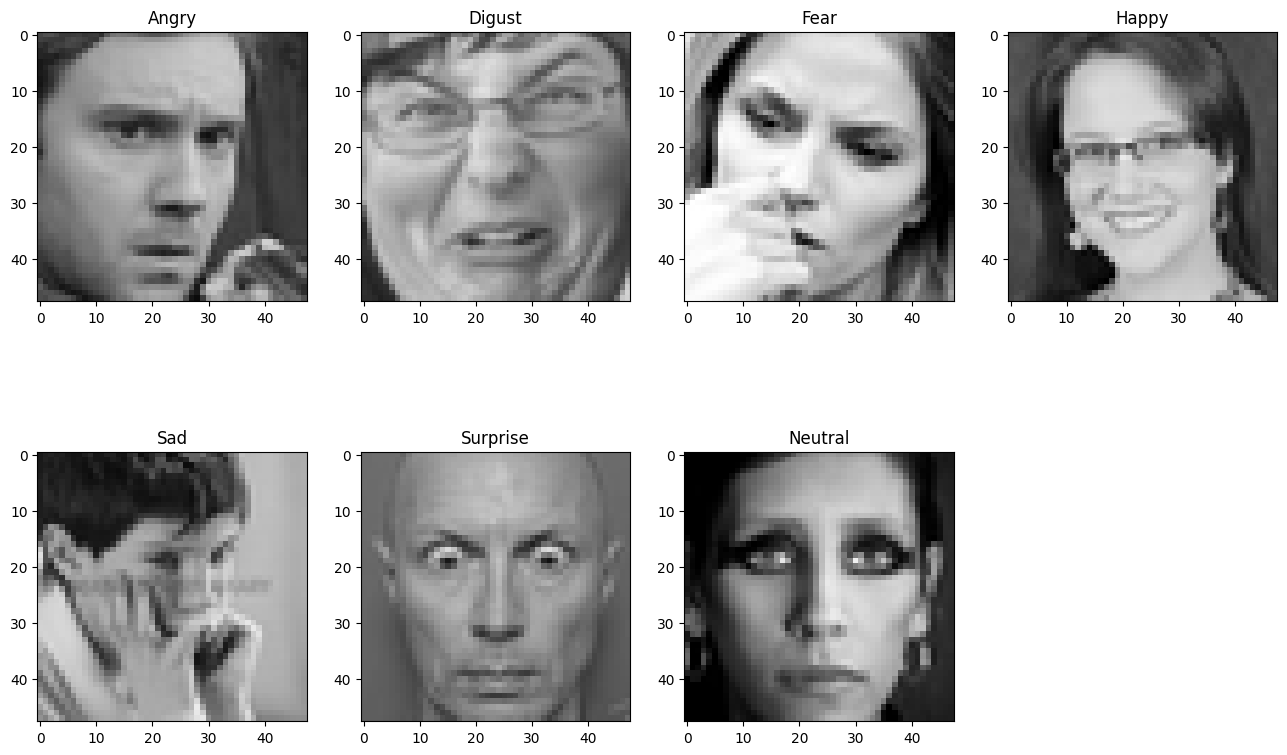
\includegraphics[width=10cm]{Images/fer2013.png}
    \caption{FER-2013 Dataset}
    \label{fig:fer2013}
\end{figure}
A dataset capable of precisely capturing a wide range of human emotions through facial expression was needed for training the model. 
Therefore, the FER-2013 \citep{challenges_in_representation_learning_facial_expression_recognition_challenge} dataset which is a well-known benchmark in the field of  \gls{fer} from the Kaggle competition platform was chosen.
A wide range of facial expressions are included in this dataset, and each of these grayscale images of faces are labelled with one of seven emotions.
This makes it suited for training \gls{fer} models.
\begin{figure}[h!]
    \centering
    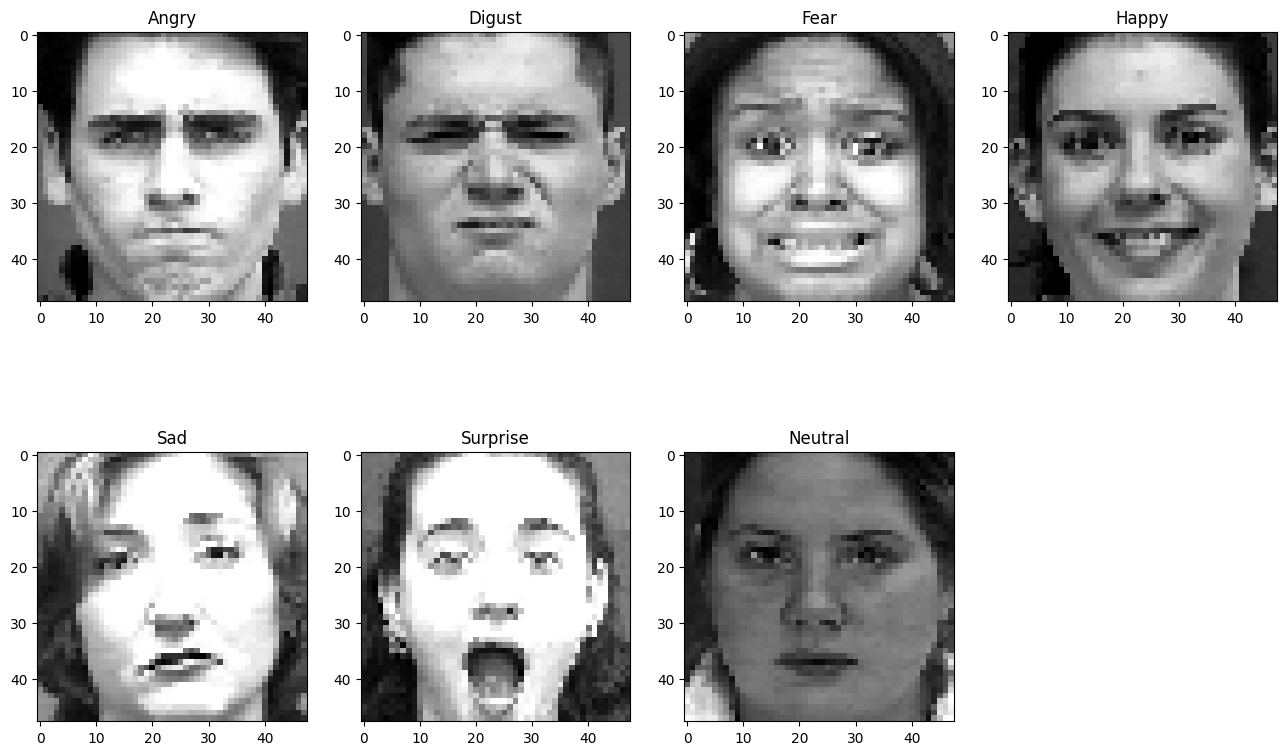
\includegraphics[width=10cm]{Images/ckextended.png}
    \caption{CK+ Dataset}
    \label{fig:ckextended}
\end{figure}
\\
\indent To increase the diversity of the data, CK+ \citep{5543262} dataset is included to the FER-2013. 
This dataset contains labelled facial expressions from varied populations and light scenarios.
This addition was to provide the models a more comprehensive learning environment by exposing them to a greater variety of face emotions and characteristics.
\begin{figure}[h!]
    \centering
    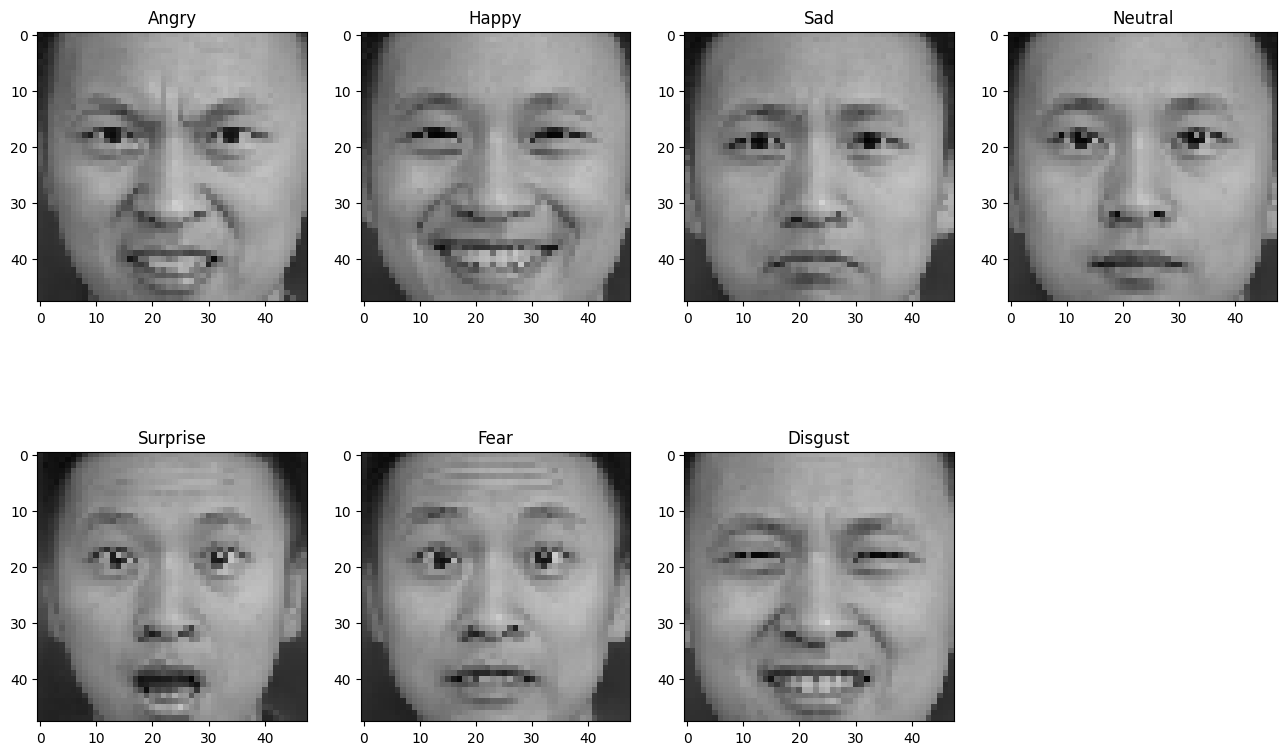
\includegraphics[width=10cm]{Images/szuemodage.png}
    \caption{SZU-EmoDage Dataset}
    \label{fig:szu-emodage}
\end{figure}
\\
\indent Moreover, SZU-EmoDage \citep{who_2022_a} dataset was also included to the collection to ensure the models are capable of identifying facial expressions on Asian faces.
With these additions, each dataset was integrated with a different set of challenges and viewpoints, which then improve the model's accuracy and practicality in real-world situation.
\paragraph{Preprocessing Steps}
Those collected data went through a series of preprocessing stages to standardize input features and optimize them for efficient \gls{ml} before training.
Even though the data were already in grayscale, all images were first converted to grayscale using the \texttt{cv2.cvtColor(image, cv2.COLOR\_BGR2GRAY)} function to ensure that all data were in grayscale in order to simplify the input data and reduce computational cost.
After conversion, all images were shrunk to 48x48 pixels.
It is because neural networks require consistent picture sizes in order to handle batch data efficiently and handle all inputs equally during the learning process.
\\
\indent Following resizing, images were flattened from a format of 2D arrays to a 1D array with 2304 elements (48x48). 
This transformation is necessary because machine learning algorithms generally require a flat array of features for each sample to be handle and analyse.
The flattened image data was then compiled into a pandas DataFrame, which made data handling and analysis in Python simpler.
Before training models, pixel values from each image were standardized to lie within the range of [0,1]. 
This normalization make sure that all input characteristics contribute equally to the model's learning because having different scale will influence the results.
\\
\indent In order to simplify the model and better match the project with its use in music recommendation, the number of emotion categories was cut down from seven to four.
The four categories were kept were `Neutral', `Happy', `Sad' and `Angry'.
These emotions are more easily applied and useful for determining musical mood.
\paragraph{Augmentation}
Keras' function `\texttt{ImageDataGenerator()}' is used to construct a strategic data augmentation process that improved the model's robustness and allowed it to generalize across a variety of face emotions and situations.
The augmentation techniques that were used included random rotation of images up to \(10^\circ\).
This mimics the natural tilts that occur in expressive moments.
Additionally, width and height shifts, which translate images by up to 10\% of their size in both directions.
This helps with situations when faces are not in the center of the frame.
\\
\indent To help the model learn to identify emotions from faces at different camera distances, random zooming was also applied to some of the images.
Moreover, the images were arbitrarily rotated horizontally so that the model could be trained on mirror copies of faces, therefore double the range of face orientations the model saw in the training.
\paragraph{Dataset Splitting}
A key phase in preparing for training and evaluation of \gls{ml} models is splitting the dataset into training, validation, and testing sets. 
The training set was composed from the `Training' data from FER-2013 and the complete CK+ dataset.
This is to increase the model's capacity to generalize across various demographic groups and emotional states by exposing it too a greater variety of facial expressions and environmental factors.
\\
\indent For validation, the `PublicTest' subset of the FER-2013 was used.
This collection is essential for adjusting the hyper-parameters of the model and for providing an unbiased evaluation of the model's fit on the training dataset.
The `PrivateTest' subset of the FER-2013 was used to do the final evaluation of the model's performance.
In addition to the training, validation, and testing data, SZU-EmoDage dataset is used specifically for transfer learning purpose. 
\subsection{Training Process}
\begin{figure}[h!] 
    \centering
\begin{minted}[frame=lines, framesep=2mm, baselinestretch=1.2, fontsize=\footnotesize, linenos]{python}
    param_grid = {
        'conv_1_filters': [32, 64],
        'conv_2_filters': [64, 96, 128],
        'conv_3_filters': [128, 192, 224],
        'conv_4_filters': [128, 160, 224, 256],
        'conv_1_kernel': [3, 5],
        'conv_2_kernel': [3, 5],
        'conv_3_kernel': [3, 5],
        'conv_4_kernel': [3, 5],
        'dropout_1': [0.1, 0.2, 0.4],
        'dropout_2': [0.0, 0.2, 0.3],
        'dropout_3': [0.0, 0.2, 0.3, 0.4],
        'dense_units': [512, 768, 1024],
        'optimizer': ['adam'],
        'batch_size': [32, 64],  
        'epochs': [10, 50, 100] 
    }
\end{minted}
    \caption{Parameter Grid}
    \label{fig:param_grid}
\end{figure}
In the training process, a common training framework was introduced for both models (Table \ref{tab:cnn-model-1} and Table \ref{tab:cnn-model-2}) to ensure consistency in the methodological approach.
But some specific adjustments to address the unique characteristics of each model is allowed.
The training process started with a thorough grid search to optimize hyper-parameters including dropout rates, kernel sizes, convolutional filter counts, and dense layer unit counts.
Both models shared the same parameter grid as Figure \ref{fig:param_grid}.
This approach made it easier to explore the configuration space in an organized way, ensuring that each model was tuned to perform optimally.
\\
\indent After searching through the parameter grid, the process focuses on configuring each model's architecture to best capture the nuances of facial expression for \gls{fer}.
Model 1 (Table \ref{tab:cnn-model-1}) has a relatively simple architecture, which require careful tuning if dropout rates and filter sizes to balance feature learning against the risk of over-fitting.
Model 2 (Table \ref{tab:cnn-model-2}) has more additional layers to capture a richer set of features before the final classification layer . 
But this led to a more thorough analysis required for the network's depth in relation to its performance on the validation set, which assisted in identifying when to add dropout and how to adjust the pooling layers.  
\\
\begin{figure}[h!] 
    \centering
\begin{minted}[frame=lines, framesep=2mm, baselinestretch=1.2, fontsize=\footnotesize, linenos]{python}
    es = EarlyStopping(monitor='val_accuracy', patience=5, restore_best_weights=True)
\end{minted}
    \caption{Early Stopping}
    \label{fig:earlystopping}
\end{figure}
\\
\indent To prevent over-fitting, early stopping mechanism, which configured as `EarlyStopping' callback (Figure \ref{fig:earlystopping}), is integrated into the training to monitor validation accuracy and automatically halt training if no improvement was detected for five consecutive epochs.
Most important of all, the callback (Figure \ref{fig:earlystopping}) was set to restore the weights form the epoch with the best validation accuracy, ensuring that the model maintained any progress made prior to the plateau.
This approach allows to train the model as long as beneficial, in the meantime, avoiding over-fitting and maintaining the optimal state achieved during training.
\\
\begin{figure}[h!] 
    \centering
\begin{minted}[frame=lines, framesep=2mm, baselinestretch=1.2, fontsize=\footnotesize, linenos]{python}
    steps_per_epoch=len(train_X) / batch_size
\end{minted}
    \caption{Steps per epoch}
    \label{fig:steps_per_epoch}
\end{figure}
\\
\indent Furthermore, the `\texttt{steps\_per\_epoch}' (Figure \ref{fig:steps_per_epoch}) parameter was calculated to ensure that each epoch processed the entire dataset.
With these techniques, early stopping and calculated epoch steps, the models were able to achieve a balance between computational prudence and strong learning.
Consequently, the models were well-positioned for dependable performance in \gls{fer}, having learned from training data efficiently and been prevented from the risk of over-fitting. 
\subsection{Model Evaluation}

\subsection{Model Comparison and Selection}
\begin{table}[ht]
    \centering
    \renewcommand{\arraystretch}{1.5}
    \begin{tabular*}{\textwidth}{@{\extracolsep{\fill}}lcr}
    \toprule
    \textbf{Property} & \textbf{Model 1} & \textbf{Model 2} \\
    \midrule
    Input shape & 48 x 48 x 1 & 48 x 48 x 1 \\
    Weight layers & 6 & 10 \\
    Conv layers & 4 & 7 \\
    Kernel size & 3x3 & 3x3 \\
    Training params & 32,113,028 & 56,303,556 \\
    Model size & - & - \\
    Accuracy (\%) & 72.36 & - \\
    \bottomrule
    \end{tabular*}
    \caption{Comparison of Model 1 with Model 2}
    \label{tab:comparison-models}
\end{table}
\section{Web Application}
\begin{figure}[h!]
    \centering
    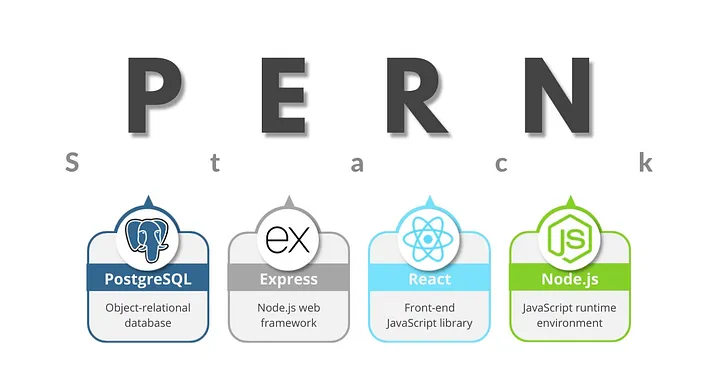
\includegraphics[width=10cm]{Images/pern.png}
    \caption{PERN Stack \citep{alves_2023_get}}
    \label{fig:pern}
\end{figure}
The web application uses the PERN stack (Figure \ref{fig:pern}), which is an acronym for PostgreSQL \citep{thepostgresqlglobaldevelopmentgroup_2019_postgresql}, Express \citep{openjsfoundation_2017_express}, React \citep{metaopensource_2024_react} and Node.js \citep{nodejs_2023_nodejs}.
This set of technologies provides a comprehensive end-to-end foundation for creating dynamic web application.
\\
\indent The frontend was built with React.js, a widely-used \gls{js} \gls{ui} framework, which was chosen for its declarative and effective method of creating \gls{ui}.
For the backend, Node.js was chosen for its non-blocking, event-driven architecture.
This architecture is well-suited for managing workloads that involve asynchronous operations, real-time applications and I/O-bound tasks.
The backend API is then constructed using Express.js, a simple and adaptable Node.js web application framework.
PostgreSQL is the chosen database system as it is well-known for its advanced features, data integrity and robustness.